\documentclass[t,11pt]{beamer}

% Lecture 6 follows the 4:3 Beamer style of the earlier course lectures.
\usepackage[T1]{fontenc}
\usepackage[utf8]{inputenc}
\usepackage{lmodern}
\usepackage{amsmath,amssymb,mathtools}
\usepackage{tikz}
\usetikzlibrary{arrows.meta,positioning,calc,fit,backgrounds}
\usepackage{array,booktabs}

\definecolor{LectureBlue}{RGB}{46,52,175}
\definecolor{BlockTitleLav}{RGB}{195,194,231}
\definecolor{BlockBodyLav}{RGB}{225,226,246}
\definecolor{SoftGray}{RGB}{115,115,115}
\useinnertheme[shadow=true]{rounded}
\setbeamercolor{normal text}{fg=black,bg=white}
\setbeamercolor{structure}{fg=LectureBlue}
\setbeamercolor{frametitle}{fg=LectureBlue,bg=white}
\setbeamercolor{block title}{fg=LectureBlue,bg=BlockTitleLav}
\setbeamercolor{block body}{fg=black,bg=BlockBodyLav}
\setbeamercolor{alerted text}{fg=LectureBlue}
\setbeamerfont{frametitle}{size=\Large,series=\mdseries}
\setbeamertemplate{blocks}[rounded][shadow=true]
\setbeamersize{text margin left=8pt,text margin right=8pt}
\setbeamertemplate{itemize items}[circle]
\setbeamertemplate{enumerate items}[circle]
\setlength{\parskip}{2pt}

\tikzset{
  state/.style={circle,draw=LectureBlue,thick,minimum size=9mm,inner sep=1pt,fill=white},
  event/.style={circle,draw=LectureBlue,thick,minimum size=10mm,inner sep=1pt,fill=white},
  flowarrow/.style={-{Latex[length=2mm]},thick,draw=black},
  dependency/.style={-{Latex[length=2mm]},thick,draw=LectureBlue},
  localbox/.style={draw=LectureBlue,rounded corners=2pt,inner sep=5pt},
  tag/.style={font=\small,fill=white,inner sep=1.4pt}
}
\newcommand{\domn}{\operatorname{dom}}
\newcommand{\Pref}{\operatorname{Pref}}
\newcommand{\lin}{\operatorname{Lin}}
\newcommand{\Sig}{\Sigma}
\newcommand{\wi}{\equiv_I}
\newcommand{\ind}{\mathrel{I}}
\newcommand{\dep}{\mathrel{D}}

\begin{document}

% =========================================================
\begin{frame}[plain]
  \vspace{1.10cm}
  \begin{center}
    {\huge\color{LectureBlue} Theory of Concurrency\par}
    \vspace{0.55cm}
    {\Large Lecture 6: Mazurkiewicz traces\par}
    \vspace{0.17cm}
    {\Large and Zielonka automata\par}
    \vspace{0.94cm}
    {\large Piotr Hofman\par}
  \end{center}
\end{frame}

\begin{frame}{Plan}
  \begin{enumerate}
    \item Problems with linear semantics.
    \item Histories.
    \item Independence relations and Mazurkiewicz traces.
    \item Dependence graphs, partial orders and Foata normal form.
    \item Trace-closed languages and their specifications.
    \item Zielonka automata and the distributed realisation theorem.
  \end{enumerate}
  \vspace{0.4cm}
  \begin{block}{Central question}
    How can we describe and implement concurrent behaviour without fixing an arbitrary order between independent events?
  \end{block}
\end{frame}


\section{Interleaving versus concurrency}

\begin{frame}{Two independent actions in an LTS}
  \begin{block}{Two local variables}
    Initially $(x,y)=(0,0)$. Action $a$ sets $x:=1$ and action $b$ sets $y:=1$.
  \end{block}
  \vspace{0.1cm}
  \begin{center}
  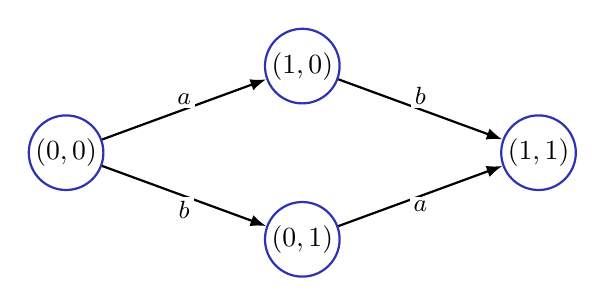
\begin{tikzpicture}[x=1cm,y=1cm]
    \node[state] (s0) at (-3,0) {$(0,0)$};
    \node[state] (sa) at (0,1.1) {$(1,0)$};
    \node[state] (sb) at (0,-1.1) {$(0,1)$};
    \node[state] (sf) at (3,0) {$(1,1)$};
    \draw[flowarrow] (s0) -- node[tag,above] {$a$} (sa);
    \draw[flowarrow] (s0) -- node[tag,below] {$b$} (sb);
    \draw[flowarrow] (sa) -- node[tag,above] {$b$} (sf);
    \draw[flowarrow] (sb) -- node[tag,below] {$a$} (sf);
  \end{tikzpicture}
  \end{center}
  \begin{block}{Two paths, the same result}
    Both $ab$ and $ba$ are executions, and both end in $(1,1)$.
  \end{block}
\end{frame}

\begin{frame}{What does an ordinary trace record?}
  \begin{block}{Interleaving semantics}
    A run of an LTS produces a word: a \emph{total order} of the actions executed.
    \[
      ab\neq ba \qquad \text{as words in }\Sigma^*.
    \]
  \end{block}
  \begin{block}{But in the preceding example}
    Neither action affects the other one's enabledness or result. The difference between $ab$ and $ba$ is only their scheduling order.
  \end{block}
  \vspace{0.12cm}
  \centering\large We want to retain necessary order, but forget irrelevant order.
\end{frame}

\begin{frame}{Interleaving explosion}
  \begin{block}{Two sequential processes}
    One process performs $a_1,a_2,\ldots,a_m$ in order; another performs $b_1,b_2,\ldots,b_n$ in order. Cross-process actions are independent.
  \end{block}
  \[
    \text{number of interleavings}=\binom{m+n}{m}.
  \]
  \begin{center}
  \begin{tabular}{c|c|c}
  First process & Second process & Interleavings\\ \hline
  $m=2$ & $n=2$ & $6$\\
  $m=4$ & $n=4$ & $70$\\
  $m=10$ & $n=10$ & $184\,756$
  \end{tabular}
  \end{center}
\end{frame}

\begin{frame}{Fairness and linearisation}
  \begin{block}{Two concurrent loops}
    Consider one process that repeatedly emits $a$, and another that repeatedly emits $b$.
    \[
    P_1: a\,a\,a\,\ldots
    \qquad \text{||}\qquad
    P_2: b\,b\,b\,\ldots
    \]
    These are independent threads of activity, not a single sequential program.
  \end{block}
  \begin{block}{A natural fairness requirement}
    The specification 
    \[
    \mathbf{G}(a\Rightarrow \mathbf{F}b) \text{does not hold for the linearisation }\ a,a,a,\cdots.
    \]
    
   \end{block}
  \begin{block}{Why this matters}
    Fairness is a property of the run as a concurrent system, not of an arbitrary total order chosen by the scheduler. Linear semantics can therefore hide behavioural defects or impose artificial ordering constraints.
  \end{block}
\end{frame}


\begin{frame}{Causality}
  \begin{block}{Independence versus dependence}
    Two events are \emph{independent} if neither one enables, disables, nor changes the effect of the other. They may be executed in either order without changing the observable outcome.
  \end{block}
  \begin{block}{Causal order}
    If one event is required to occur before another because it influences its result or enables it, then the first is a \emph{cause} of the second. This gives a partial order, not a total one.
  \end{block}
  \begin{center}
  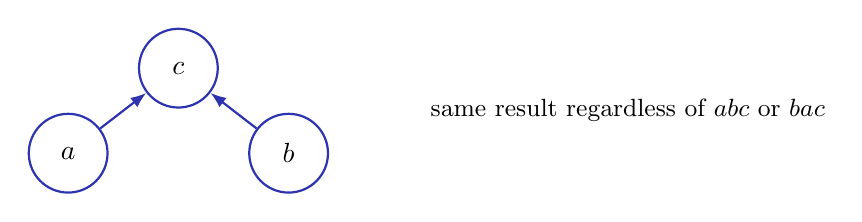
\begin{tikzpicture}[x=1.4cm,y=.9cm]
    \node[event] (a) at (0,0) {$a$};
    \node[event] (b) at (2,0) {$b$};
    \node[event] (c) at (1,1.2) {$c$};
    \draw[dependency] (a) -- (c);
    \draw[dependency] (b) -- (c);
    \node[font=\small,anchor=west] at (3.2,0.6) {same result regardless of $abc$ or $bac$};
  \end{tikzpicture}
  \end{center}
 
\end{frame}


\begin{frame}{Why linear semantics is not enough}
  \begin{block}{A scheduler chooses an order, but not necessarily a causal one}
    An execution of a concurrent system is often represented as a word
    \[
      a_1a_2\cdots a_n.
    \]
  \end{block}
  \begin{block}{Problems}
    \begin{itemize}
      \item The word order records arbitrary scheduling choices, not essential causality.
      \item Fairness may require that a process is eventually scheduled, even if its actions are not the next ones in a fixed linearisation.
      \item Exponential blow-up appears because independent actions generate many equivalent serialisations.
    \end{itemize}
  \end{block}
  \centering\large The semantics should keep only the order that matters for behaviour.
\end{frame}

\begin{frame}{Distributed logs (Another problem)}
  \begin{block}{Problem with logging}
    In distributed systems, each machine writes its local events with its own clock. A global log is often assembled later by merging timestamps, but different clocks may drift and messages may be delayed or reordered.
  \end{block}
  \begin{block}{Example: Patriot missile failure 1991}
    \begin{itemize}
      \item After 100 hours, the radar clock drifted by 0.34 seconds.
      \item This small error shifted the tracked position of a Scud by roughly 500 meters.
      \item The missile missed its target; 28 soldiers were killed.
    \end{itemize}
  \end{block}

\end{frame}

% \begin{frame}{Histories}
%   \begin{block}{Processes and their alphabets}
%     Let $P=\{p_1,p_2,p_3\}$, with local alphabets
%     \[
%       \Sigma_{p_1}=\{a,c\},\quad \Sigma_{p_2}=\{b,c\},\quad \Sigma_{p_3}=\{d\}.
%     \]
%     An action shared by processes is communication: they synchronize by executing that same action. Here $c$ is one event involving both $p_1$ and $p_2$.
%   \end{block}
%   \begin{center}
%   \begin{tikzpicture}[x=.9cm,y=.7cm]
%     \draw[black,thick] (-2,1.2) -- (2,1.2);
%     \draw[black,thick] (-2,0.2) -- (2,0.2);
%     \draw[black,thick] (-2,-0.8) -- (2,-0.8);
%     \node[font=\small,anchor=east] at (-2,1.2) {$p_1$};
%     \node[font=\small,anchor=east] at (-2,0.2) {$p_2$};
%     \node[font=\small,anchor=east] at (-2,-0.8) {$p_3$};
%     \node[event,minimum size=8mm] (p1a) at (-0.6,1.2) {$a$};
%     \node[event,minimum size=8mm] (p1c) at (1.3,1.2) {$c$};
%     \node[event,minimum size=8mm] (p2b) at (-0.6,0.2) {$b$};
%     \node[event,minimum size=8mm] (p2c) at (1.3,0.2) {$c$};
%     \node[event,minimum size=8mm] (p3d) at (0.3,-0.8) {$d$};
%     \draw[dependency] (p1a) -- (p1c);
%     \draw[dependency] (p2b) -- (p2c);
%     \draw[thick,dashed] (p1c) -- node[tag,right,font=\scriptsize] {same event} (p2c);
%   \end{tikzpicture}
%   \end{center}

% \end{frame}

% \begin{frame}{When is swapping actions incorrect?}
%   \begin{block}{Shared variable}
%     Let $a$ assign $x:=1$ and $b$ assign $x:=2$.
%   \end{block}
%   \[
%   \begin{aligned}
%     x=0&\xrightarrow{a}x=1\xrightarrow{b}x=2,\\[5pt]
%     x=0&\xrightarrow{b}x=2\xrightarrow{a}x=1.
%   \end{aligned}
%   \]
%   \begin{block}{Dependence matters}
%     The order of $a$ and $b$ changes the outcome. They cannot be declared independent.
%   \end{block}
%\end{frame}


% \begin{frame}{Histories (Approach 1)}


% \begin{block}{What should be dependnet?}
% Actions in the same process are dependent. For them, we have causality relation.
% \end{block}

%    \begin{block}{Dependence and independence}
%     Actions are dependent iff their process domains intersect; disjoint domains mean independence. Thus $a$ and $b$ are independent, as is $d$ from $a,b,c$.
%   \end{block}

% \end{frame}


\begin{frame}{Histories (Approach 1)}
\begin{block}{Assumptions:}
\begin{enumerate}
 \item We have $k$ processes running in parallel. 
 \item Each action of the process$_i$ has a unique name in $\Sigma_i$.
 \item They communicate via rendezvous.
 \item If $a$ belongs to the alphabets of a few systems then all
 of them perform it synchronously.  
\end{enumerate}
\end{block}

\visible<2->{
\begin{block}{}
We consider a monoid $M=\Sigma_1^*\times \Sigma_2^*\times
\ldots \Sigma_k^*$ with concatenation defined via coordinates $(u_1,u_2,\ldots, u_k)+(w_1,w_2,\ldots, w_k)=
(u_1 w_1,u_2 w_2,\ldots, u_k w_k)$.
\end{block}
}
\visible<3->{
\begin{block}{}
Let $\Sigma=\Sigma_1\cup\Sigma_2\cup\ldots \Sigma_k$. For 
$a\in \Sigma$ we define $u_a\in M$ as $(x_1,x_2,\ldots,x_k)$
where $x_i=\varepsilon$ if $a\not\in \Sigma_i$ and
$x_i=a$ if $a\in \Sigma_i$. We call the set of $u_a$ elementary histories.
\end{block}
}


\end{frame}




\begin{frame}{Histories}

\begin{block}{The history is}
a submonoid of $M$ generated by elementary histories.
\end{block}
\visible<2->{
\begin{block}{Projection $\pi_i$}
For a word $w\in \Sigma^*$ its projection $\pi_i$ is a
word $w_i\in \Sigma_i^*$ obtained from $w$ by removing letters 
not in $\Sigma_i$.
\end{block}
}
\visible<3->{
\begin{block}{Projection $\pi$}
For a word $w\in \Sigma^*$ its projection $\pi$ is an element of the monoid $M$
$(\pi_1(w),\pi_2(w),\ldots,\pi_k(w))$.
\end{block}
}
\visible<4->{
\begin{block}{Mathematical structure of histories}
\begin{itemize}
 \item Monoid structure.
 \item Projections goes form strings to the monoid of histories.
\end{itemize}
\end{block}
}

\end{frame}





% =========================================================


% =========================================================
\section{Mazurkiewicz traces}

\newcommand{\Ind}{I}
\newcommand{\Dep}{D}


\begin{frame}{Independence and dependence alphabets (Approach 2)}
  \begin{block}{Definition}
    A \emph{concurrent alphabet} is $(\Sigma,I)$, where $\Sigma$ is finite and
    \[
       \Ind\subseteq\Sigma\times\Sigma
    \]
    is a \textbf{symmetric, irreflexive} independence relation.
  \end{block}
  \begin{block}{Dependence relation}
    \[
      D=(\Sigma\times\Sigma)\setminus I.
    \]
    Dependence is symmetric and reflexive.
  \end{block}
  \vspace{0.1cm}
  We read $a\ind b$ as ``$a$ and $b$ may commute'', and $a\dep b$ as ``their order must be retained''.
\end{frame}

\begin{frame}{A running dependence alphabet}
  \[
    \Sigma=\{a,b,c\},\qquad I=\{(a,b),(b,a)\}.
  \]
  \begin{center}
  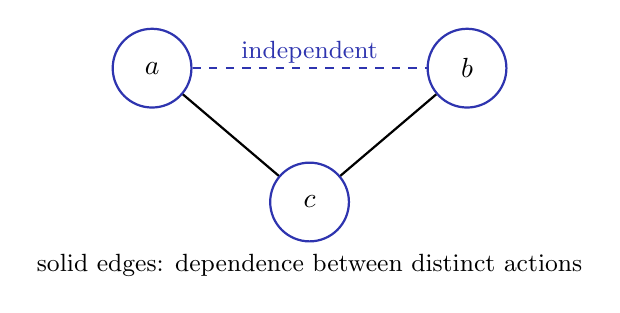
\begin{tikzpicture}[scale=1]
    \node[event] (a) at (-2,0) {$a$};
    \node[event] (b) at (2,0) {$b$};
    \node[event] (c) at (0,-1.7) {$c$};
    \draw[LectureBlue,thick,dashed] (a) -- node[tag,above] {independent} (b);
    \draw[thick] (a) -- (c);
    \draw[thick] (b) -- (c);
    \node[font=\small] at (0,-2.5) {solid edges: dependence between distinct actions};
  \end{tikzpicture}
  \end{center}
  \begin{block}{Important distinction}
    $a\ind b$, while $a\dep c$ and $b\dep c$. Dependence need not be transitive; every action also depends on itself.
  \end{block}
\end{frame}

\begin{frame}{Swapping independent neighbours}
  \begin{block}{Elementary equivalence}
    If $a\ind b$, then for every $u,v\in\Sigma^*$,
    \[
      uabv \;\longleftrightarrow\; ubav.
    \]
    Let $\equiv_I$ be the equivalence relation generated by these swaps.
  \end{block}
  \begin{block}{Example: $I=\{(a,b),(b,a)\}$}
    \[
    \underbrace{abc\equiv_I bac}_{\text{swap }a,b},
    \qquad
    \underbrace{abc\not\equiv_I acb}_{\text{cannot swap }b,c}.
    \]
  \end{block}
  Swaps act on \emph{adjacent} positions; a sequence of swaps may be needed.
\end{frame}

\begin{frame}{Mazurkiewicz traces}
  \begin{block}{Definition}
    A \emph{Mazurkiewicz trace} is an equivalence class of words under $\equiv_I$:
    \[
      [w]_I=\{v\in\Sigma^*:v\equiv_I w\}.
    \]
  \end{block}
  \begin{block}{Our example}
    For $I=\{(a,b),(b,a)\}$,
    \[
      [abc]_I=\{abc,bac\},\qquad [acb]_I=\{acb\}.
    \]
  \end{block}
  \vspace{0.25cm}
  A trace represents an execution \emph{up to permutations of independent actions}.
\end{frame}

\begin{frame}{Why traces form a monoid}
  \begin{block}{Congruence property}
    Swapping independent neighbours remains valid inside larger words:
    \[
      u\equiv_Iu',\quad v\equiv_Iv'
      \quad\Longrightarrow\quad uv\equiv_Iu'v'.
    \]
  \end{block}
  \begin{block}{Trace monoid}
    \[
      M(\Sigma,I)=\Sigma^*/{\equiv_I},\qquad
      [u]_I\cdot[v]_I=[uv]_I.
    \]
    The empty word $\varepsilon$ induces the identity element $[\varepsilon]_I$.
  \end{block}
  \vspace{0.15cm}
  Concatenation of traces is well-defined, independently of the chosen word representatives.
\end{frame}

\begin{frame}{Two extreme forms of independence}
  \begin{block}{No independent distinct actions: $I=\varnothing$}
    No swaps are allowed. Every trace consists of one word:
    \[
      M(\Sigma,\varnothing)=\Sigma^*.
    \]
  \end{block}
  \begin{block}{All distinct actions independent}
    $I=\{(a,b):a\neq b\}$. Words are equivalent exactly when each letter occurs equally often.
    \[
      abc\equiv_I bca\equiv_I cab.
    \]
    The trace remembers only the numbers of occurrences of actions.
  \end{block}
  Most concurrent alphabets lie between these extremes.
\end{frame}

\begin{frame}{From word languages to trace languages}
  \begin{block}{Quotient map}
    \[
       q:\Sigma^*\longrightarrow M(\Sigma,I),\qquad q(w)=[w]_I.
    \]
    A word language $L\subseteq\Sigma^*$ induces the trace language
    \[
       q(L)=\{[w]_I:w\in L\}.
    \]
  \end{block}

\end{frame}

%=================
\section{Comparison of traces and histories}

\begin{frame}{}

\begin{block}{}
By $u \div a$ we mean right cancellation of $a$ from $u$. For $u$ beeing a string
it is defined as follows:
$$ u \div a = \begin{cases}
\varepsilon \ for\ u=\varepsilon,\\
v\ for\ u=va\\
(v\div a)b \ for \ u=vb\ where \ b\neq a
\end{cases}  $$
\end{block}
 
\begin{lemma}
  $u \equiv w \implies u \div a \equiv w \div a$ for any $a\in \Sigma$.
\end{lemma}

\visible<2->{ 
\begin{block}{}
A dependency morphism w.r.t. $D$ is any homomorphism from the monoid of strings over $\Sigma$
on to another monoid such that
\begin{enumerate}
\item[A1] $\phi(w)=\phi(\varepsilon) \implies w=\varepsilon;$
\item[A2]$(a,b)\in\Ind \implies \phi(ab)=\phi(ba);$
\item[A3] $\phi(ua)=\phi(v) \implies \phi(u)=\phi(v\div a);$
\item[A4] $\phi(ua)=\phi(vb)\land a\neq b \implies (a,b)\in \Ind$
\end{enumerate} 
\end{block}
}
\end{frame}



\begin{frame}{}
We want to prove $3$ theorems.

\begin{theorem}
Let $\phi$ and $\psi$ are two dependency morphism going from $\Sigma^*$ to monoids $M$ and $N$. Then $M$ and $N$ are isomorphic. 
\end{theorem}

\visible<2->{
\begin{lemma}
Let $\phi$ be a dependency morphism, $u,v\in \Sigma^*$ $a,b\in \Sigma$. If $\phi(ua)=\phi(vb)$ and $a\neq b$ then there exists $w\in \Sigma^*$ such that $\phi(u)=\phi(wb)$ and $\phi(v)=\phi(wa)$.
\end{lemma}
}

\visible<3->{
\begin{theorem}
Canonical homomorphism of string into Mazurkiewicz traces is a dependency morphism.  
\end{theorem}
}

\visible<4->{
\begin{theorem}
Canonical homomorphism of string into histories is a dependency morphism.  
\end{theorem}
}
\end{frame}





% =========================================================
\section{Partial-order representation}

\begin{frame}{From total orders to partial orders}
  \begin{center}
  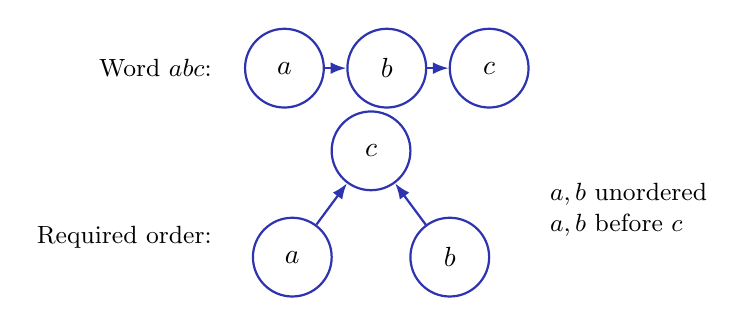
\begin{tikzpicture}[x=1cm,y=1cm]
    \node[font=\small,anchor=east] at (-2.5,0.6) {Word $abc$:};
    \node[event] (wa) at (-1.7,.6) {$a$};
    \node[event] (wb) at (-.4,.6) {$b$};
    \node[event] (wc) at (.9,.6) {$c$};
    \draw[dependency] (wa) -- (wb);
    \draw[dependency] (wb) -- (wc);
    \node[font=\small,anchor=east] at (-2.5,-1.55) {Required order:};
    \node[event] (pa) at (-1.6,-1.8) {$a$};
    \node[event] (pb) at (.4,-1.8) {$b$};
    \node[event] (pc) at (-.6,-.45) {$c$};
    \draw[dependency] (pa) -- (pc);
    \draw[dependency] (pb) -- (pc);
    \node[font=\small,align=left,anchor=west] at (1.55,-1.2) {$a,b$ unordered\\$a,b$ before $c$};
  \end{tikzpicture}
  \end{center}
  \begin{block}{Idea}
    A word imposes an order on \emph{all} positions. A dependence graph keeps only the order forced by dependent actions.
  \end{block}
\end{frame}

\begin{frame}{Dependence graph of a word}
  \begin{block}{Construction}
    Let $w=a_1a_2\cdots a_n$. Create a distinct event vertex for each position:
    Add an edge $i\to j$ whenever
    \[
       i<j\quad\text{and}\quad (a_i,a_j)\in D.
    \]
    Take the reflexive transitive closure to obtain the order $\leq_w$.
  \end{block}
  \begin{block}{Important}
    Vertices are \textbf{occurrences}, not action names. In particular, two occurrences of the same action are ordered because $(a,a)\in D$.
  \end{block}
\end{frame}

\begin{frame}{Dependence graph: $abc$}
  \[
      I=\{(a,b),(b,a)\},\qquad w=abc.
  \]
  \begin{center}
  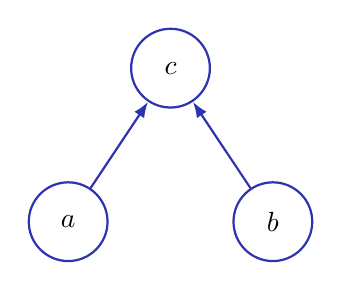
\begin{tikzpicture}[x=1cm,y=1cm]
    \node[event] (a) at (-1.3,-1.4) {$a$};
    \node[event] (b) at (1.3,-1.4) {$b$};
    \node[event] (c) at (0,0.55) {$c$};
    \draw[dependency] (a) -- (c);
    \draw[dependency] (b) -- (c);
    \node[font=\small] at (0,-2.0) {%The Hasse diagram of the dependence order
    };
  \end{tikzpicture}
  \end{center}
  \begin{block}{Linearizations}
    The labelled partial order has exactly two linearizations:
    \[
       \lin(E_w,\leq_w,\lambda)=\{abc,bac\}.
    \]
  \end{block}
\end{frame}

\begin{frame}{Independent labels can still be ordered}
  \[
     I=\{(a,b),(b,a)\},\qquad w=acb.
  \]
  \begin{center}
  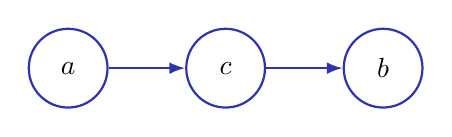
\begin{tikzpicture}
    \node[event] (a) at (-2,0) {$a$};
    \node[event] (c) at (0,0) {$c$};
    \node[event] (b) at (2,0) {$b$};
    \draw[dependency] (a) -- (c);
    \draw[dependency] (c) -- (b);
  \end{tikzpicture}
  \end{center}
  \begin{block}{Transitive causality}
    Although $a\ind b$, the order contains $a<c<b$ because both actions depend on $c$.
  \end{block}
  \vspace{0.2cm}
  Independence of \emph{action labels} does not guarantee that two particular \emph{occurrences} are unordered.
\end{frame}

\begin{frame}{Fundamental characterisation of traces}
  \begin{block}{Theorem}
    For finite words $u,v\in\Sigma^*$,
    \[
       u\equiv_Iv
       \quad\Longleftrightarrow\quad
       \text{their labelled dependence posets are isomorphic}.
    \]
  \end{block}
  \begin{block}{Proof idea: $\Rightarrow$}
    Swapping adjacent independent events preserves every order constraint between dependent occurrences.
  \end{block}
  \begin{block}{Proof idea: $\Leftarrow$}
    Any two linear extensions of a finite poset are connected by adjacent swaps of incomparable events. In a dependence poset, incomparable events have independent labels.
  \end{block}
\end{frame}

\begin{frame}{Lexicographic normal form}
  \begin{block}{Choose an order on the alphabet}
    Fix a total order, for example $a<b<c$. Each trace contains finitely many words, so it has a unique lexicographically least representative.
    \[
      \operatorname{lexmin}([w]_I)
      =\min_{\mathrm{lex}}\{v\in\Sigma^*:v\equiv_Iw\}.
    \]
  \end{block}
  \begin{block}{Example}
    With $I=\{(a,b),(b,a)\}$,
    \[
       [abc]_I=\{abc,bac\},\qquad
       \operatorname{lexmin}([abc]_I)=abc.
    \]
  \end{block}
  The chosen word is canonical, but it is still a \emph{total order}: it does not display which events could have happened concurrently.
\end{frame}

\begin{frame}{Foata normal form: concurrent layers}
  \begin{block}{Canonical representation}
    Repeatedly take all minimal events of the dependence poset, record them as one layer, and remove them. Every layer consists of pairwise independent actions.
  \end{block}
  \[
      w=abcabc,\qquad I=\{(a,b),(b,a)\}.
  \]
  \begin{center}
  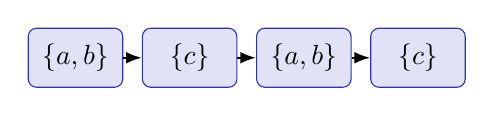
\begin{tikzpicture}[x=1.45cm,y=.75cm]
    \node[draw=LectureBlue,rounded corners=3pt,fill=BlockBodyLav,minimum width=1.2cm,minimum height=.75cm] (k0) at (0,0) {$\{a,b\}$};
    \node[draw=LectureBlue,rounded corners=3pt,fill=BlockBodyLav,minimum width=1.2cm,minimum height=.75cm] (k1) at (1,0) {$\{c\}$};
    \node[draw=LectureBlue,rounded corners=3pt,fill=BlockBodyLav,minimum width=1.2cm,minimum height=.75cm] (k2) at (2,0) {$\{a,b\}$};
    \node[draw=LectureBlue,rounded corners=3pt,fill=BlockBodyLav,minimum width=1.2cm,minimum height=.75cm] (k3) at (3,0) {$\{c\}$};
    \draw[flowarrow] (k0) -- (k1);
    \draw[flowarrow] (k1) -- (k2);
    \draw[flowarrow] (k2) -- (k3);
  \end{tikzpicture}
  \end{center}
  \begin{block}{Foata normal form}
    \[
       \{a,b\}\;\{c\}\;\{a,b\}\;\{c\}.
    \]
    These layers are uniquely determined by a finite trace.
  \end{block}
\end{frame}

\begin{frame}{Foata layers are not time slots}
  \[
    \Sigma=\{a,b,c\},\qquad I=\{(a,b),(b,a),(b,c),(c,b)\}.
  \]
  Thus $a\dep c$, while $b$ is independent of both $a$ and $c$.
  \begin{block}{One trace, two linearizations}
    The words $abc$ and $acb$ differ only by swapping the independent actions $b,c$.
    Their dependence order has just one constraint: $a<c$.
  \end{block}
  \begin{center}
    \[
      \operatorname{Foata}(abc)=\operatorname{Foata}(acb)
      =\{a,b\}\;\{c\}.
    \]
  \end{center}
  \begin{block}{How to read the layers}
    The layers give events their dependence depth; they are not strict time slots.
    Here $b$ is in the first layer but may occur after $c$, as the linearization $acb$ shows.
  \end{block}
\end{frame}


\begin{frame}{Foata form and lexicographic form}
  \begin{center}
  \begin{tabular}{>{\raggedright\arraybackslash}p{.27\textwidth}|>{\raggedright\arraybackslash}p{.30\textwidth}|>{\raggedright\arraybackslash}p{.30\textwidth}}
    & \textbf{Lexicographic} & \textbf{Foata}\\ \hline
    Representation & One chosen word & A sequence of concurrent layers\\
    Captures concurrency & No; serialises a trace & Yes; independent events can share a layer\\
    Canonical? & Yes, after fixing an alphabet order & Yes, from the dependence order\\
    Useful for & Comparing or storing traces as words & Seeing causal depth and available parallelism
  \end{tabular}
  \end{center}
  \begin{block}{Same trace, different emphasis}
    For $[abc]_I=\{abc,bac\}$ with $a\ind b$, the lexicographic form is $abc$, while the Foata form is $\{a,b\}\{c\}$.
  \end{block}
\end{frame}


\begin{frame}{What information does a trace preserve?}
  \begin{block}{Preserved}
    Event occurrences, action labels, and the ordering constraints induced by dependence.
  \end{block}
  \begin{block}{Forgotten}
    The chosen interleaving of incomparable events. A trace does not record physical durations or a schedule.
  \end{block}
  \begin{block}{Not represented by one trace}
    Branching choices between different possible executions of an entire system.
  \end{block}
\end{frame}

% =========================================================
\section{Trace languages}



\begin{frame}{Trace-closed languages}
  \begin{block}{Definition}
    A language $L\subseteq\Sigma^*$ is \emph{$I$-closed} (or \emph{trace-closed}) if
    \[
      u\in L\ \text{and}\ u\equiv_Iv
      \quad\Longrightarrow\quad v\in L.
    \]
    Equivalently, $uabv\in L$ iff $ubav\in L$ whenever $a\ind b$.
  \end{block}
  \begin{block}{Example}
    Let $\Sigma=\{a,b,c\}$, with $a\ind b$ and both dependent on $c$. Let
    \[
      A=(a+b)^*,\qquad R=AaAbA+AbAaA,\qquad L=(Rc)^*A.
    \]
    $R$ consists of words containing both letters; each $c$ closes one such block. Swapping neighbouring $a,b$ preserves membership in $L$.
  \end{block}
\end{frame}

\begin{frame}{A requirement that is not trace-closed}
  \[
     \Sigma=\{a,b\},\qquad a\ind b,\qquad L=\{ab\}.
  \]
  \begin{block}{Problem}
    $ab\in L$, but $ba\notin L$, although $ab\equiv_Iba$.
  \end{block}
  \[
    q^{-1}\bigl(q(L)\bigr)=\{ab,ba\}\neq L.
  \]
  \begin{block}{Interpretation}
    The specification explicitly requires $a$ before $b$, so these two actions cannot simultaneously be treated as independent for this requirement.
  \end{block}
\end{frame}

\begin{frame}{Why an LTS should satisfy diamonds}
  \begin{block}{Commutation property}
    For independent $a,b$, whenever
    $s\xrightarrow{a}s_1\xrightarrow{b}t$,
    there must be some $s_2$ with
    $s\xrightarrow{b}s_2\xrightarrow{a}t$.
  \end{block}
  \begin{center}
  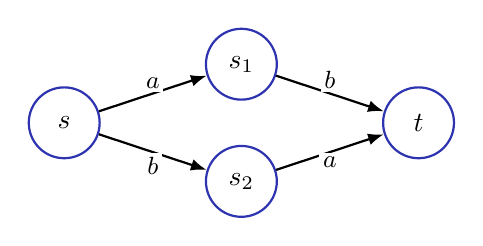
\begin{tikzpicture}[x=1cm,y=.62cm]
    \node[state] (s) at (-2.25,0) {$s$};
    \node[state] (sa) at (0,1.2) {$s_1$};
    \node[state] (sb) at (0,-1.2) {$s_2$};
    \node[state] (t) at (2.25,0) {$t$};
    \draw[flowarrow] (s) -- node[tag,above] {$a$} (sa);
    \draw[flowarrow] (s) -- node[tag,below] {$b$} (sb);
    \draw[flowarrow] (sa) -- node[tag,above] {$b$} (t);
    \draw[flowarrow] (sb) -- node[tag,below] {$a$} (t);
  \end{tikzpicture}
  \end{center}
  \begin{block}{Consequence}
    If this replacement is always possible along runs, the finite trace language of the LTS is $I$-closed.
  \end{block}
\end{frame}

\begin{frame}{From regular specifications to distributed machines}
  \begin{block}{Finite-state specification}
    Regularity means that a finite automaton can recognise the word language $L\subseteq\Sigma^*$. This is a finite-state description of the allowed executions.
  \end{block}
  \begin{block}{Concurrency-respecting specification}
    If $L$ is $I$-closed, acceptance depends on the trace, not on which order independent actions happened to take.
  \end{block}
  \begin{block}{Implementation question}
    Can such a specification be implemented with finite local states, so each action accesses only the processes that participate in it?
  \end{block}
  \centering\textbf{Zielonka's theorem says yes for every regular, $I$-closed language.}
\end{frame}

% =========================================================
\section{Zielonka automata}

\begin{frame}{Distributed alphabets}
  \begin{block}{Definition}
    Let $P$ be a finite set of processes. A \emph{distributed alphabet} provides
    \[
       \domn:\Sigma\longrightarrow 2^P\setminus\{\varnothing\}.
    \]
    The set $\domn(a)$ contains exactly the processes that participate in $a$.
  \end{block}
  \begin{center}
    \begin{tabular}{c|c|l}
      action & domain & meaning\\ \hline
      $a$ & $\{p\}$ & local action of $p$\\
      $b$ & $\{q\}$ & local action of $q$\\
      $c$ & $\{p,q\}$ & synchronization of $p$ and $q$
    \end{tabular}
  \end{center}
  \[
      a\ind b\quad\Longleftrightarrow\quad \domn(a)\cap\domn(b)=\varnothing.
  \]
\end{frame}

\begin{frame}{Why process domains explain independence}
  \begin{center}
  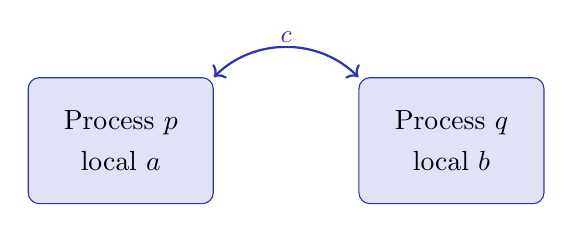
\begin{tikzpicture}[x=1cm,y=1cm]
    \node[draw=LectureBlue,rounded corners,fill=BlockBodyLav,minimum width=2.35cm,minimum height=1.6cm,align=center] (p) at (-2.1,0) {Process $p$\\[3pt]local $a$};
    \node[draw=LectureBlue,rounded corners,fill=BlockBodyLav,minimum width=2.35cm,minimum height=1.6cm,align=center] (q) at (2.1,0) {Process $q$\\[3pt]local $b$};
    \draw[LectureBlue,thick,<->] (p.north east) to[out=45,in=135] node[tag,above] {$c$} (q.north west);
  \end{tikzpicture}
  \end{center}
  \begin{block}{Local and shared actions}
    $a$ changes only the state of $p$, while $b$ changes only the state of $q$. Action $c$ involves both processes and can coordinate their states.
  \end{block}
  \vspace{0.15cm}
  Disjoint process domains give a structural reason for the commutation of actions.
\end{frame}

\begin{frame}{Zielonka automata: local states}
  \begin{block}{Global configuration}
    Each process $p\in P$ has a finite local state space $Q_p$ and initial state $q_p^0$. A global configuration is a tuple
    \[
        (q_p)_{p\in P}\in\prod_{p\in P}Q_p.
    \]
  \end{block}
  \begin{block}{Action semantics}
    An action $a$ reads and updates \emph{only} the states of processes in $\domn(a)$. All other local states remain unchanged.
  \end{block}
  \vspace{0.18cm}
  A shared action is one atomic synchronization step of all its participating processes.
\end{frame}

\begin{frame}{Formal definition of a Zielonka automaton}
  \begin{block}{Deterministic finite asynchronous automaton}
    A Zielonka automaton consists of finite local state sets $(Q_p)_{p\in P}$, an initial tuple $q^0$, a set of accepting global states
    \[
      F\subseteq\prod_{p\in P}Q_p,
    \]
    and, for each $a\in\Sigma$, a \emph{partial} local update function
    \[
      \delta_a:\prod_{p\in\domn(a)}Q_p
      \rightharpoonup\prod_{p\in\domn(a)}Q_p.
    \]
  \end{block}
  \begin{block}{Reading a word}
    Execute its actions from $q^0$ when their local updates are defined. A word is accepted if the final global tuple belongs to $F$.
  \end{block}
\end{frame}

\begin{frame}{A two-process Zielonka automaton}
  \begin{block}{Local states and initial configuration}
    Processes $p$ and $q$ each have local state space $\{0,1\}$, with initial state $0$.
    Thus the initial global configuration is $(0,0)$.
  \end{block}
  \begin{center}
  \begin{tabular}{c|c|l}
    action & domain & partial local update\\ \hline
    $a$ & $\{p\}$ & $0\mapsto1$ on $p$\\
    $b$ & $\{q\}$ & $0\mapsto1$ on $q$\\
    $c$ & $\{p,q\}$ & $(1,1)\mapsto(0,0)$
  \end{tabular}
  \end{center}
  \begin{block}{Reading the updates}
    Actions $a$ and $b$ are enabled only when their process is in state $0$; they are independent.
    The synchronization $c$ is enabled only when both processes are in state $1$ and resets both.
  \end{block}
  Every global state is accepting. The next slide shows the resulting global LTS.
\end{frame}

\begin{frame}{Global LTS of the Zielonka automaton}
  \begin{center}
  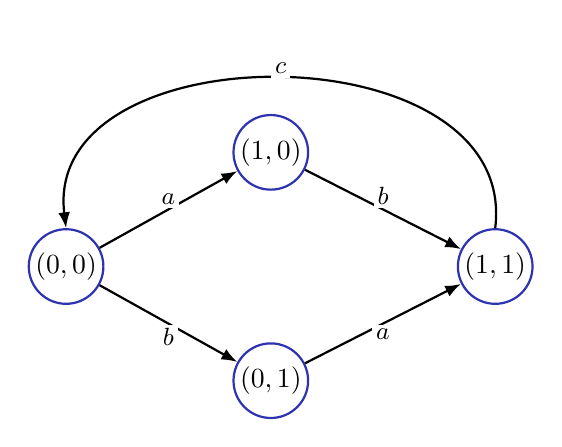
\begin{tikzpicture}[x=1cm,y=1cm]
    \node[state] (s0) at (-3,0) {$(0,0)$};
    \node[state] (sa) at (-.4,1.45) {$(1,0)$};
    \node[state] (sb) at (-.4,-1.45) {$(0,1)$};
    \node[state] (sf) at (2.45,0) {$(1,1)$};
    \draw[flowarrow] (s0) -- node[tag,above] {$a$} (sa);
    \draw[flowarrow] (s0) -- node[tag,below] {$b$} (sb);
    \draw[flowarrow] (sa) -- node[tag,above] {$b$} (sf);
    \draw[flowarrow] (sb) -- node[tag,below] {$a$} (sf);
    \draw[flowarrow] (sf.north) to[out=83,in=97,looseness=1.2] node[tag,above] {$c$} (s0.north);
  \end{tikzpicture}
  \end{center}
  \begin{block}{Global view, local implementation}
    The diagram is an ordinary LTS, but its transitions are generated from local updates and one shared synchronization.
  \end{block}
\end{frame}

\begin{frame}{The language recognised by the example}
  \begin{block}{Accept all reachable global states}
    Take $F=Q_p\times Q_q$. Then the accepted language consists of valid prefixes of rounds with one $a$, one $b$, and a closing $c$:
    \[
       L=\Pref\bigl(((ab+ba)c)^*\bigr).
    \]
  \end{block}
  \begin{center}
  \begin{tabular}{l|l}
    accepted & not accepted\\ \hline
    $\varepsilon,\ a,\ b,\ ab,\ ba$ & $c$\\
    $abc,\ bac,\ abcabc$ & $acb,\ aabc$
  \end{tabular}
  \end{center}
  \begin{block}{Trace closure}
    Every exchange of adjacent $a,b$ preserves acceptance: $abc$ and $bac$ are two linearizations of one accepted trace.
  \end{block}
\end{frame}

\begin{frame}{Independence is built into the automaton}
  \begin{block}{Disjoint local updates commute}
    If $\domn(a)\cap\domn(b)=\varnothing$, the two updates read and modify disjoint coordinates.
    \[
       q\xrightarrow{a}q_1\xrightarrow{b}q'
       \quad\Longleftrightarrow\quad
       q\xrightarrow{b}q_2\xrightarrow{a}q'.
    \]
  \end{block}
  \begin{block}{Consequence}
    Every word accepted by a Zielonka automaton can be replaced by any $I$-equivalent word without changing the final global state. Its language is $I$-closed.
  \end{block}
  \vspace{0.15cm}
  This follows from the architecture, not from a separately imposed commutation axiom.
\end{frame}

\begin{frame}{Zielonka's theorem}
  \begin{block}{Theorem (Zielonka, 1987)}
    Fix a finite distributed alphabet $(\Sigma,\domn)$ and its induced independence relation $I$.

    If a language $L\subseteq\Sigma^*$ is
    \begin{itemize}
      \item regular, and
      \item $I$-closed,
    \end{itemize}
    then $L$ is recognised by a \textbf{finite deterministic Zielonka automaton} over this distributed alphabet.
  \end{block}
  \begin{block}{Conversely}
    Every language recognised by a finite Zielonka automaton (with global final states) is regular and $I$-closed.
  \end{block}
\end{frame}



\begin{frame}{What does Zielonka's theorem say?}
  \begin{block}{Specification}
    A centralised finite automaton can specify a global behaviour language, provided it is closed under the independence relation.
  \end{block}
  \begin{block}{Implementation}
    There exists a finite automaton with separate local states: every action uses only the local states of its participating processes.
  \end{block}
  \begin{block}{Limit of the result}
    The theorem is an expressiveness result. It does \emph{not} promise a small distributed implementation. The construction and its size bounds are nontrivial.
  \end{block}
\end{frame}

\begin{frame}{Why local projections are not enough}
  \begin{block}{Two processes and a trace-closed language}
    Let $\domn(a)=\{p\}$, $\domn(b)=\{q\}$, and $\domn(c)=\{p,q\}$, so $a\ind b$. Consider
    \[
      L=\{acb,\ bca\}.
    \]
    This language is $I$-closed: the independent actions $a,b$ are never adjacent in either word.
  \end{block}
  \begin{block}{Project onto each process}
    \[
      \pi_p(L)=\{ac,ca\},\qquad \pi_q(L)=\{cb,bc\}.
    \]
    A construction accepting whenever both local projections are accepted also accepts $w=abc$, since
    \[
      \pi_p(w)=ac\in\pi_p(L),\qquad \pi_q(w)=bc\in\pi_q(L).
    \]
    But $abc\notin L$.
  \end{block}
\end{frame}

\begin{frame}{The missing information: correlation}
  \begin{block}{What the projections forget}
    In $acb$, process $p$ performs $ac$ while $q$ performs $cb$. In $bca$, they perform $ca$ and $bc$. Separate projections also allow the mixed combination $ac$ with $bc$, producing the spurious word $abc$.
  \end{block}
  \begin{block}{Scope of the counterexample}
    This refutes the rule ``accept iff every process accepts its projection,'' not Zielonka's theorem. In this example, local states can retain which projected word occurred, and a suitable set of \emph{global} accepting tuples can accept the two intended combinations while rejecting the mixed one.
  \end{block}
  \begin{block}{Why the theorem is nontrivial}
    A distributed automaton must preserve enough information about which local behaviours can occur together. The theorem guarantees a finite construction that does so; simply recognising each projection independently does not.
  \end{block}
\end{frame}





\begin{frame}{Proof}
Blackbord. 
\end{frame}



\begin{frame}{References}
  \begin{thebibliography}{10}
    \bibitem{Zielonka87}
    W. Zielonka.
    \newblock \emph{Notes on finite asynchronous automata}.
    \newblock RAIRO -- Theoretical Informatics and Applications, 21(2):99--135, 1987.

    \bibitem{BookTraces}
    V. Diekert and G. Rozenberg (eds.).
    \newblock \emph{The Book of Traces}.
    \newblock World Scientific, 1995.

    \bibitem{BaierKatoen}
    C. Baier and J.-P. Katoen.
    \newblock \emph{Principles of Model Checking}.
    \newblock MIT Press, 2008.
  \end{thebibliography}
\end{frame}

\end{document}
